\chapter{Mobile Networks}
\begin{figure}[htbp]
   \centering
   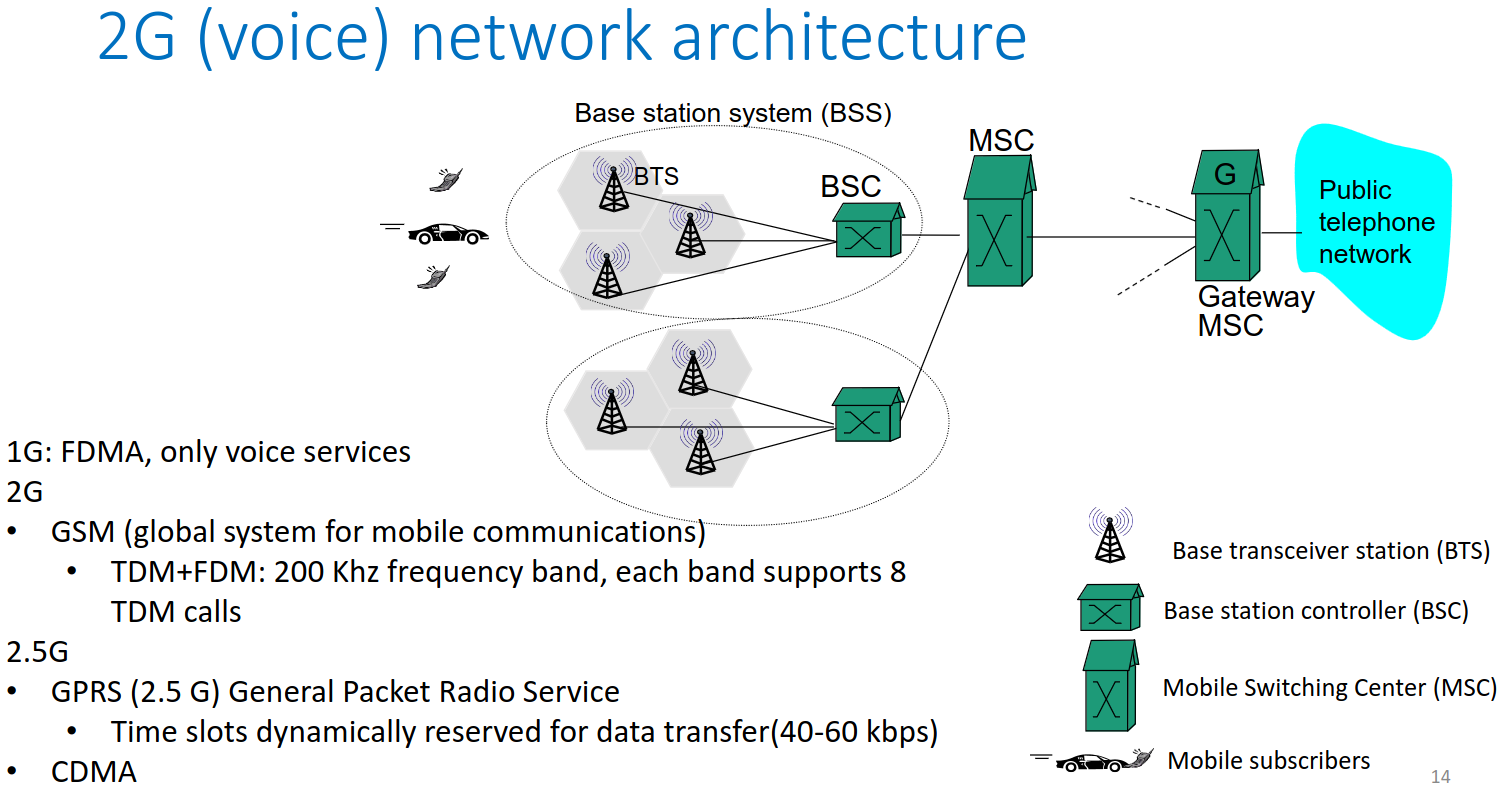
\includegraphics[width=0.45\columnwidth]{images/2g_architecture.png}
   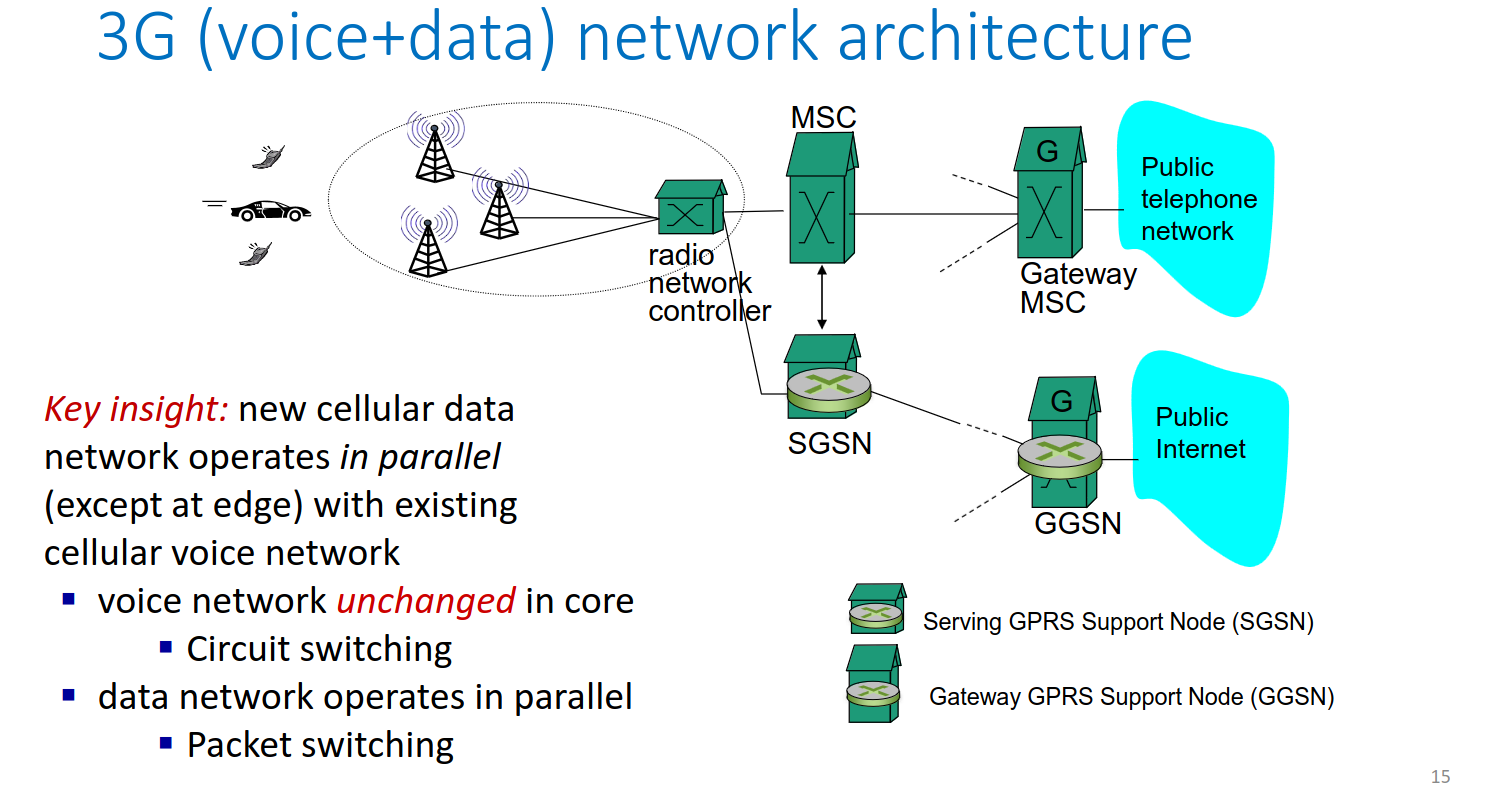
\includegraphics[width=0.45\columnwidth]{images/3g_architecture.png}\\
   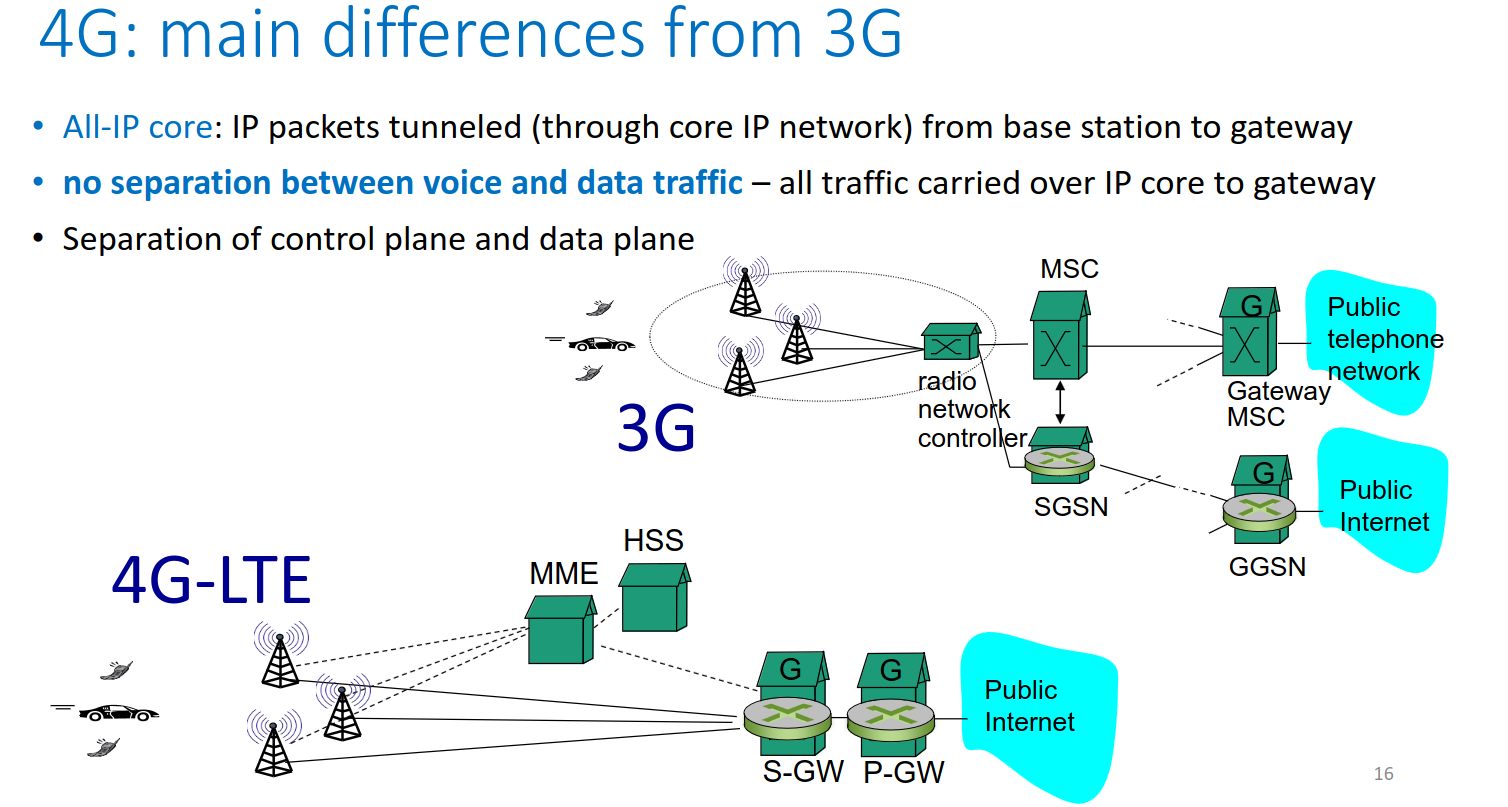
\includegraphics[width=0.45\columnwidth]{images/4g_architecture_3gcomp.png}
   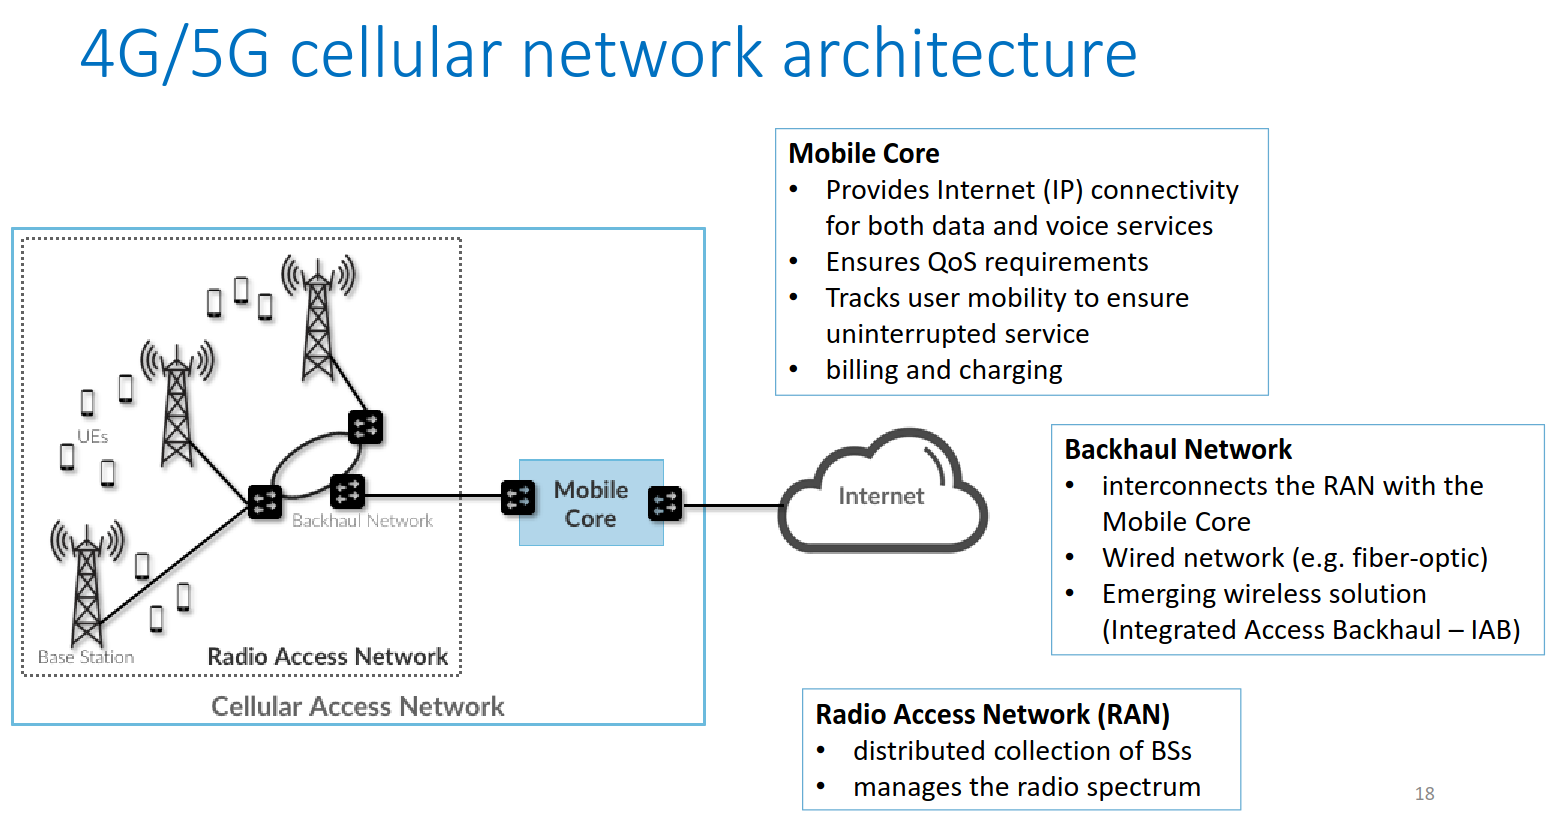
\includegraphics[width=0.45\columnwidth]{images/5g_architecture.png}

   \caption{Mobile Networks architectures}
   \label{fig:mobile_architectures}
\end{figure}

The key point in \textbf{3G} is the introduction of a data service, operating in parallel with voice network, which forced the important modifications to the architecture.

In \textbf{4G} also the voice traffic uses \textit{packet switching}, instead of circuit switching.

\section{4G Focus}

\begin{figure}[htbp]
   \centering
   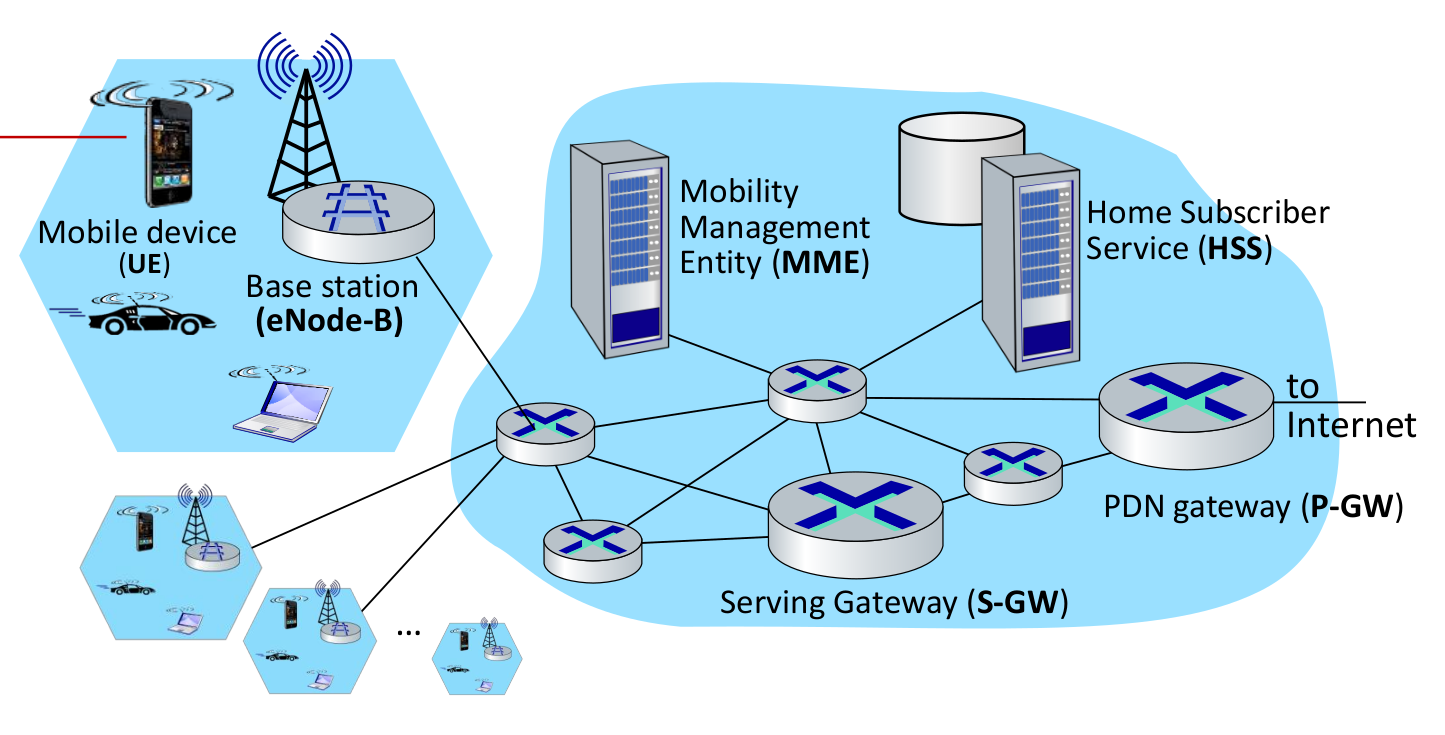
\includegraphics{images/4g_architecture.png}
   \caption{4G architecture key elements}
   \label{fig:4g_architecture}
\end{figure}

\begin{itemize}
   \item Mobile End devices
   \item Base station
   \begin{itemize}
      \item Creates device-specific IP tunnels from
      the mobile device to gateways
      \item At the edge of carrier's network
   \end{itemize}
   \item Home Subscriber Server (HSS)
   \begin{itemize}
      \item A database that contains all subscriber-related information
      \item Stores info about mobile devices for which the HSS's network is their ``home network''
      \item Works with MME in device authentication
   \end{itemize}
   \item Mobility Management Entity (MME)
   \begin{itemize}
      \item Device authentication (device-to-network, network- to-device) coordinated with mobile home network HSS
      \item Mobile device management:
      \begin{itemize}
         \item Device handover between cells
         \item Tracking/paging device location
         \end{itemize}
      \item Path (tunneling) setup from mobile device to P-GW
   \end{itemize}
   \item Serving Gateway (SGW)
   \begin{itemize}
      \item Forwards data packets between to and from RAN (Radio Access Network)
      \item Responsible for inter-enB handover, and provides mobility between 4G and other networks such as between 2G/3G and PG-W
   \end{itemize}
   \item Packet Data Network Gateway (PGW)
   \begin{itemize}
      \item A gateway to mobile cellular network
      \item Looks like any other internet router and provides NAT services
   \end{itemize}
\end{itemize}

\framedt{Control vs Data plane}{
   \textbf{Control plane} includes routing protocols such as BGP and all the processes which handle and determine how data packets should be forwarded.
   
   \textbf{Data plane} instead handles the transport of host/application data, and performs the actually forwarding of packets.
   
   \textit{\footnotesize``Think of the control plane as being like the stoplights that operate at the intersections of a city. Meanwhile, the data plane (or the forwarding plane) is more like the cars that drive on the roads, stop at the intersections, and obey the stoplights''}
   \href{https://www.cloudflare.com/it-it/learning/network-layer/what-is-the-control-plane/}{Cloudflare Data/Control plane}
}


\section{Mobility}
\begin{figure}[htbp]
   \centering
   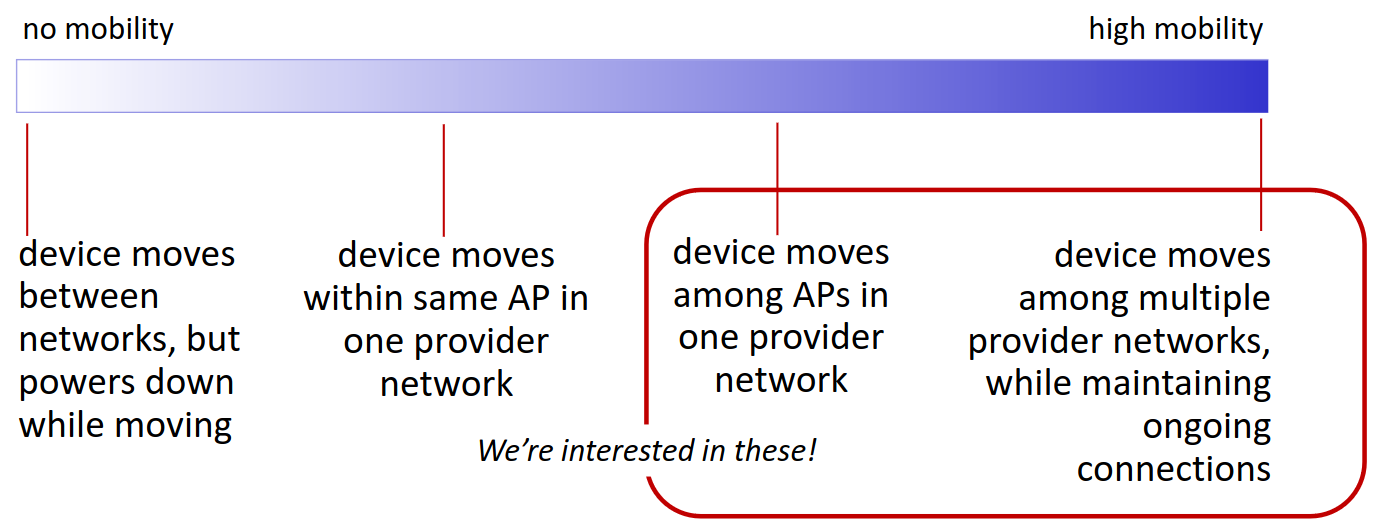
\includegraphics{images/mobility.png}
   \caption{Mobility}
   \label{fig:mobility}
\end{figure}
To handle devices' mobility there must be a home network to rely onto.
\begin{figure}[htbp]
   \centering
   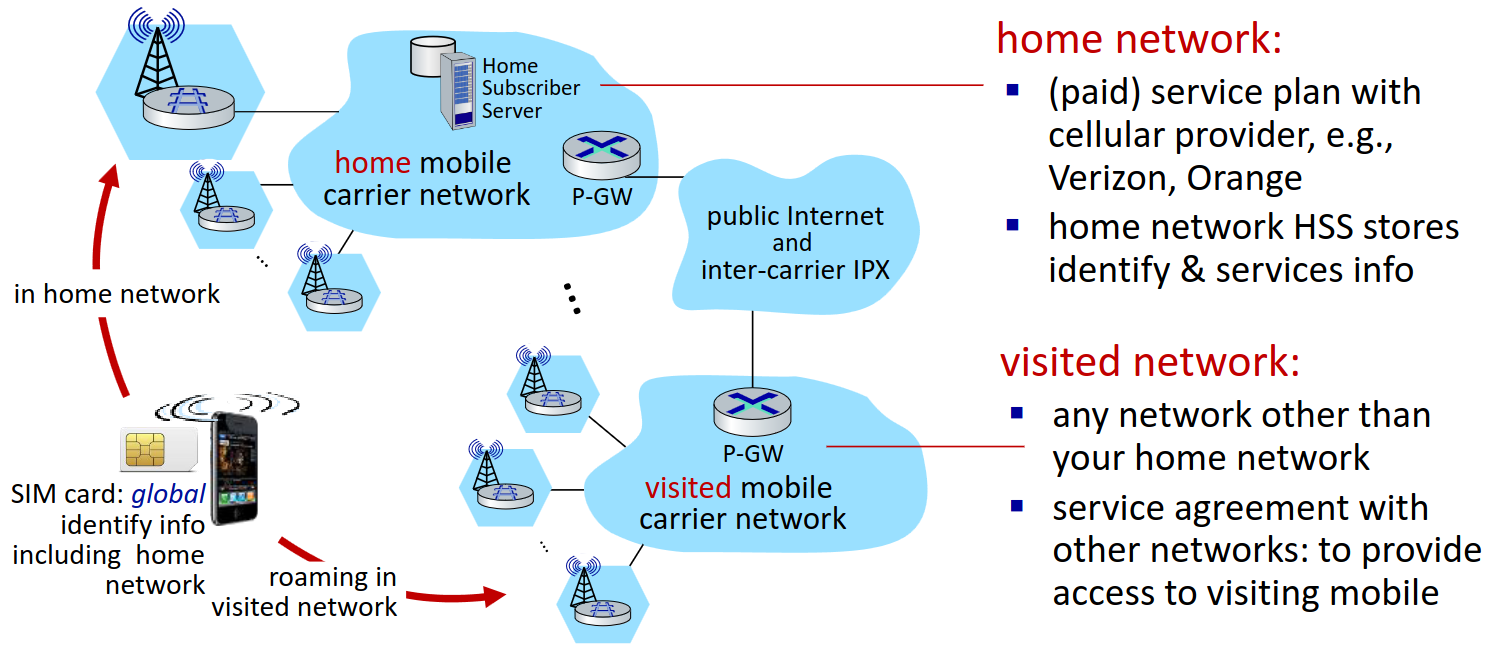
\includegraphics[width=0.45\columnwidth]{images/homenetwork.png}
   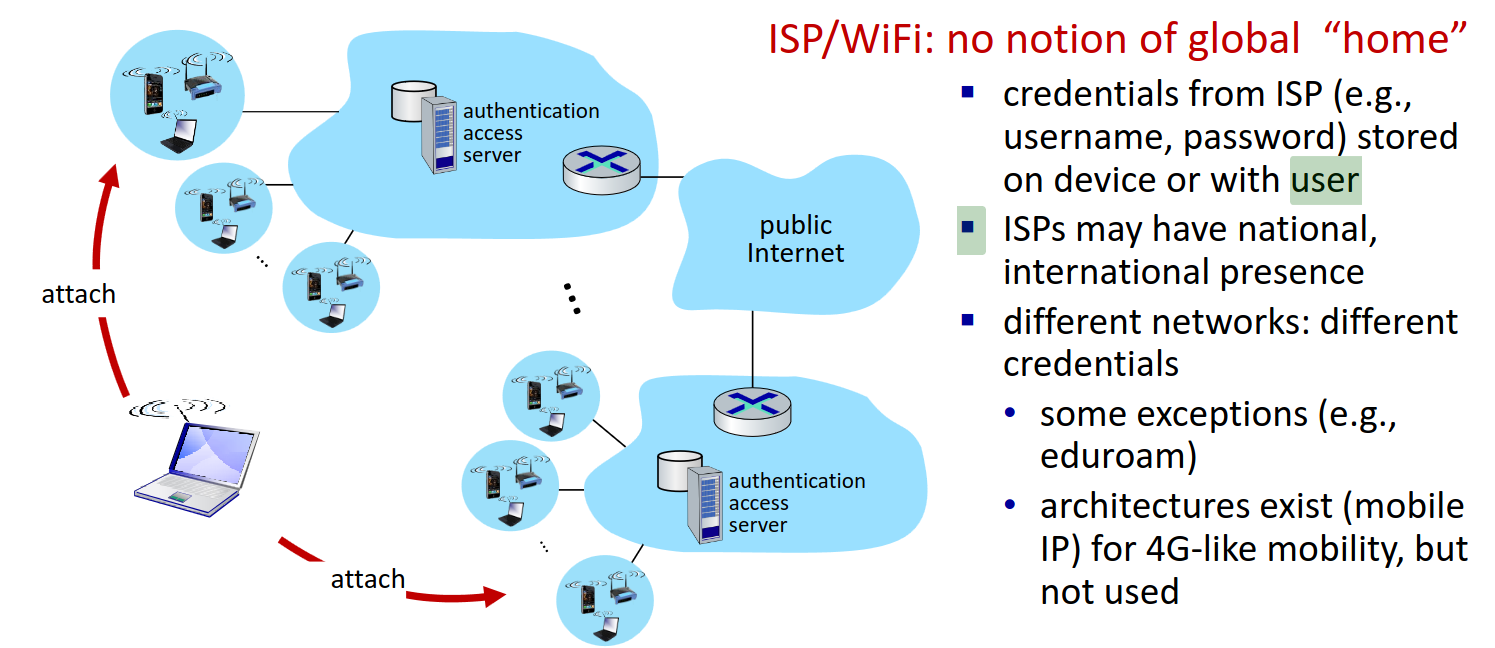
\includegraphics[width=0.45\columnwidth]{images/homenetwork2.png}\\
   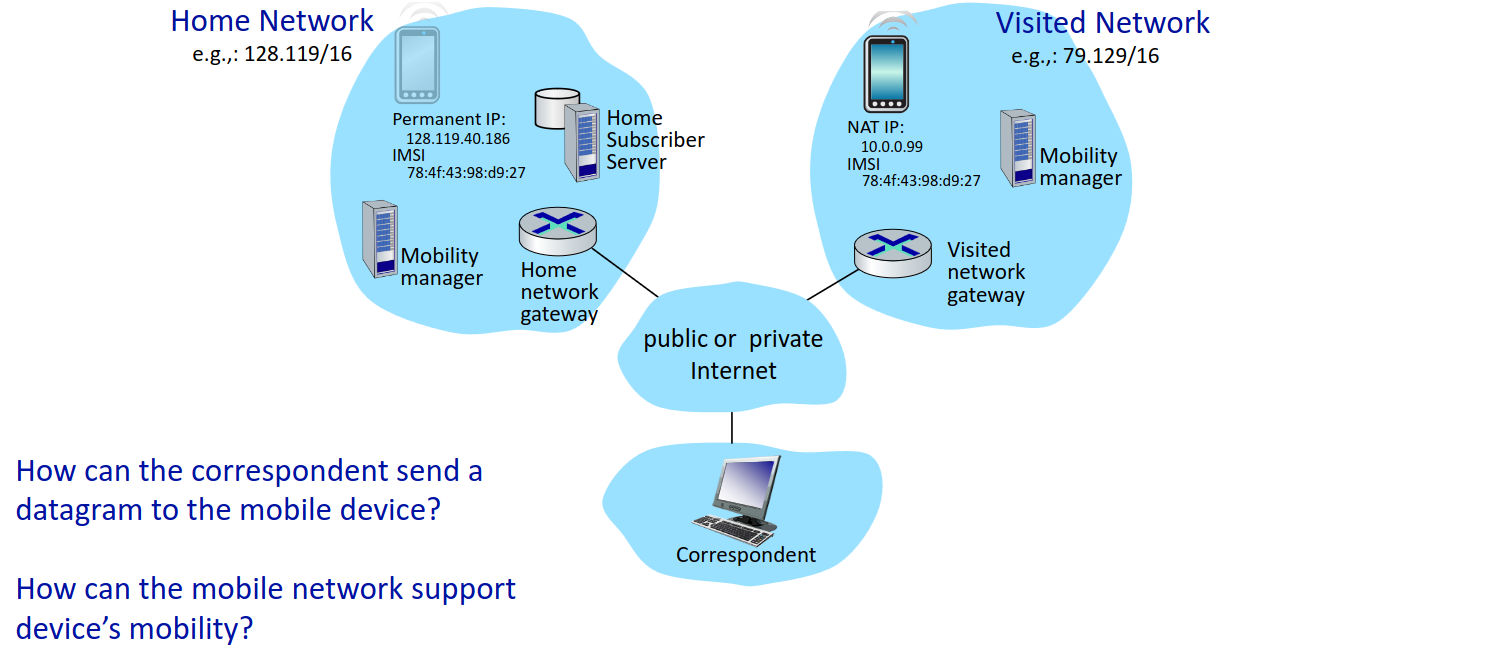
\includegraphics[width=0.45\columnwidth]{images/homenetwork3.png}
   \caption{Home and visited Networks}
   \label{fig:homenetwork}
\end{figure}

With respect to the questions posed in the third image in Fig. \ref{fig:homenetwork}, data being send from a device to a mobile one may be routed in three ways.
\begin{enumerate}
   \item 
   The first is the canonical routing, using IP addresses and routing tables, \ul{but it is not a feasible scenario for billions of devices}.
   \item The other possibility is to rely on the edge of \textbf{home} and \textbf{visited} networks instead.
   \begin{enumerate}
      \item \textbf{Direct routing}\\
      Sender gets foreign address of mobile, send directly to mobile
      \item \textbf{Indirect routing}\\
      Communication from sender to mobile goes through home network, then forwarded to remote mobile
   \end{enumerate}
\end{enumerate}

We will focus on the second possibility, which is the most common in mobile networks.
First of all the home network needs to know the current location of the mobile device,
% which is done by the \textbf{Home Location Register} (HLR) and the \textbf{Visitor Location Register} (VLR).
so first it associates with the Mobility Management Entity (MME) of the visited network to authenticate the device, which in turn informs the Home Subscriber Server (HSS) of the device's location.
\begin{figure}[htbp]
   \centering
   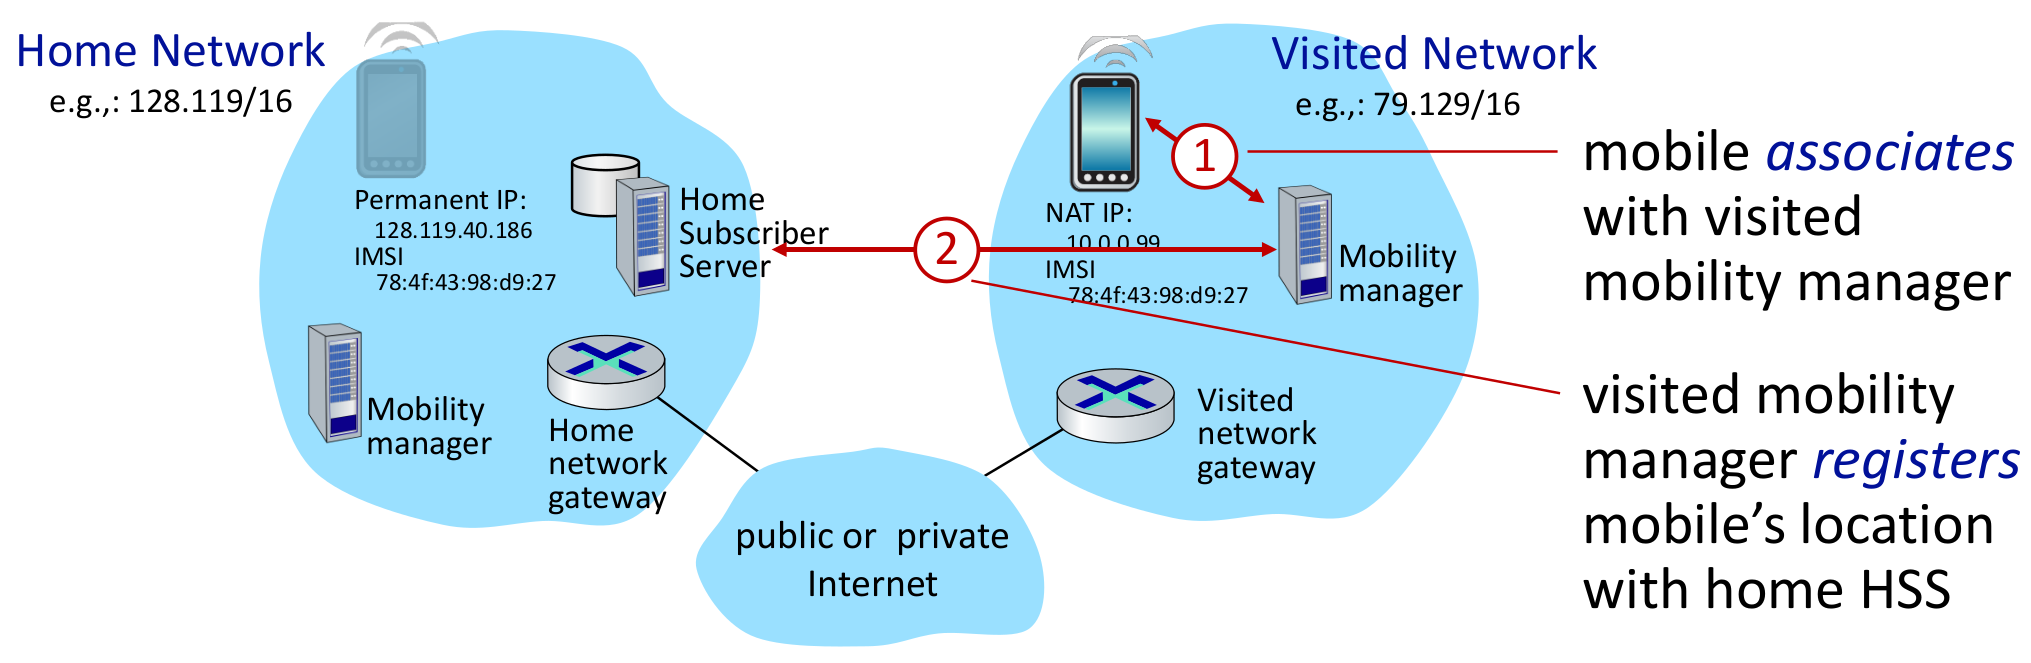
\includegraphics{images/mobility_homenetwork.png}
   % \caption{}
   \label{fig:mobility_homenetwork}
\end{figure}

\subsection{Indirect Routing}

\begin{figure}[htbp]
   \centering
   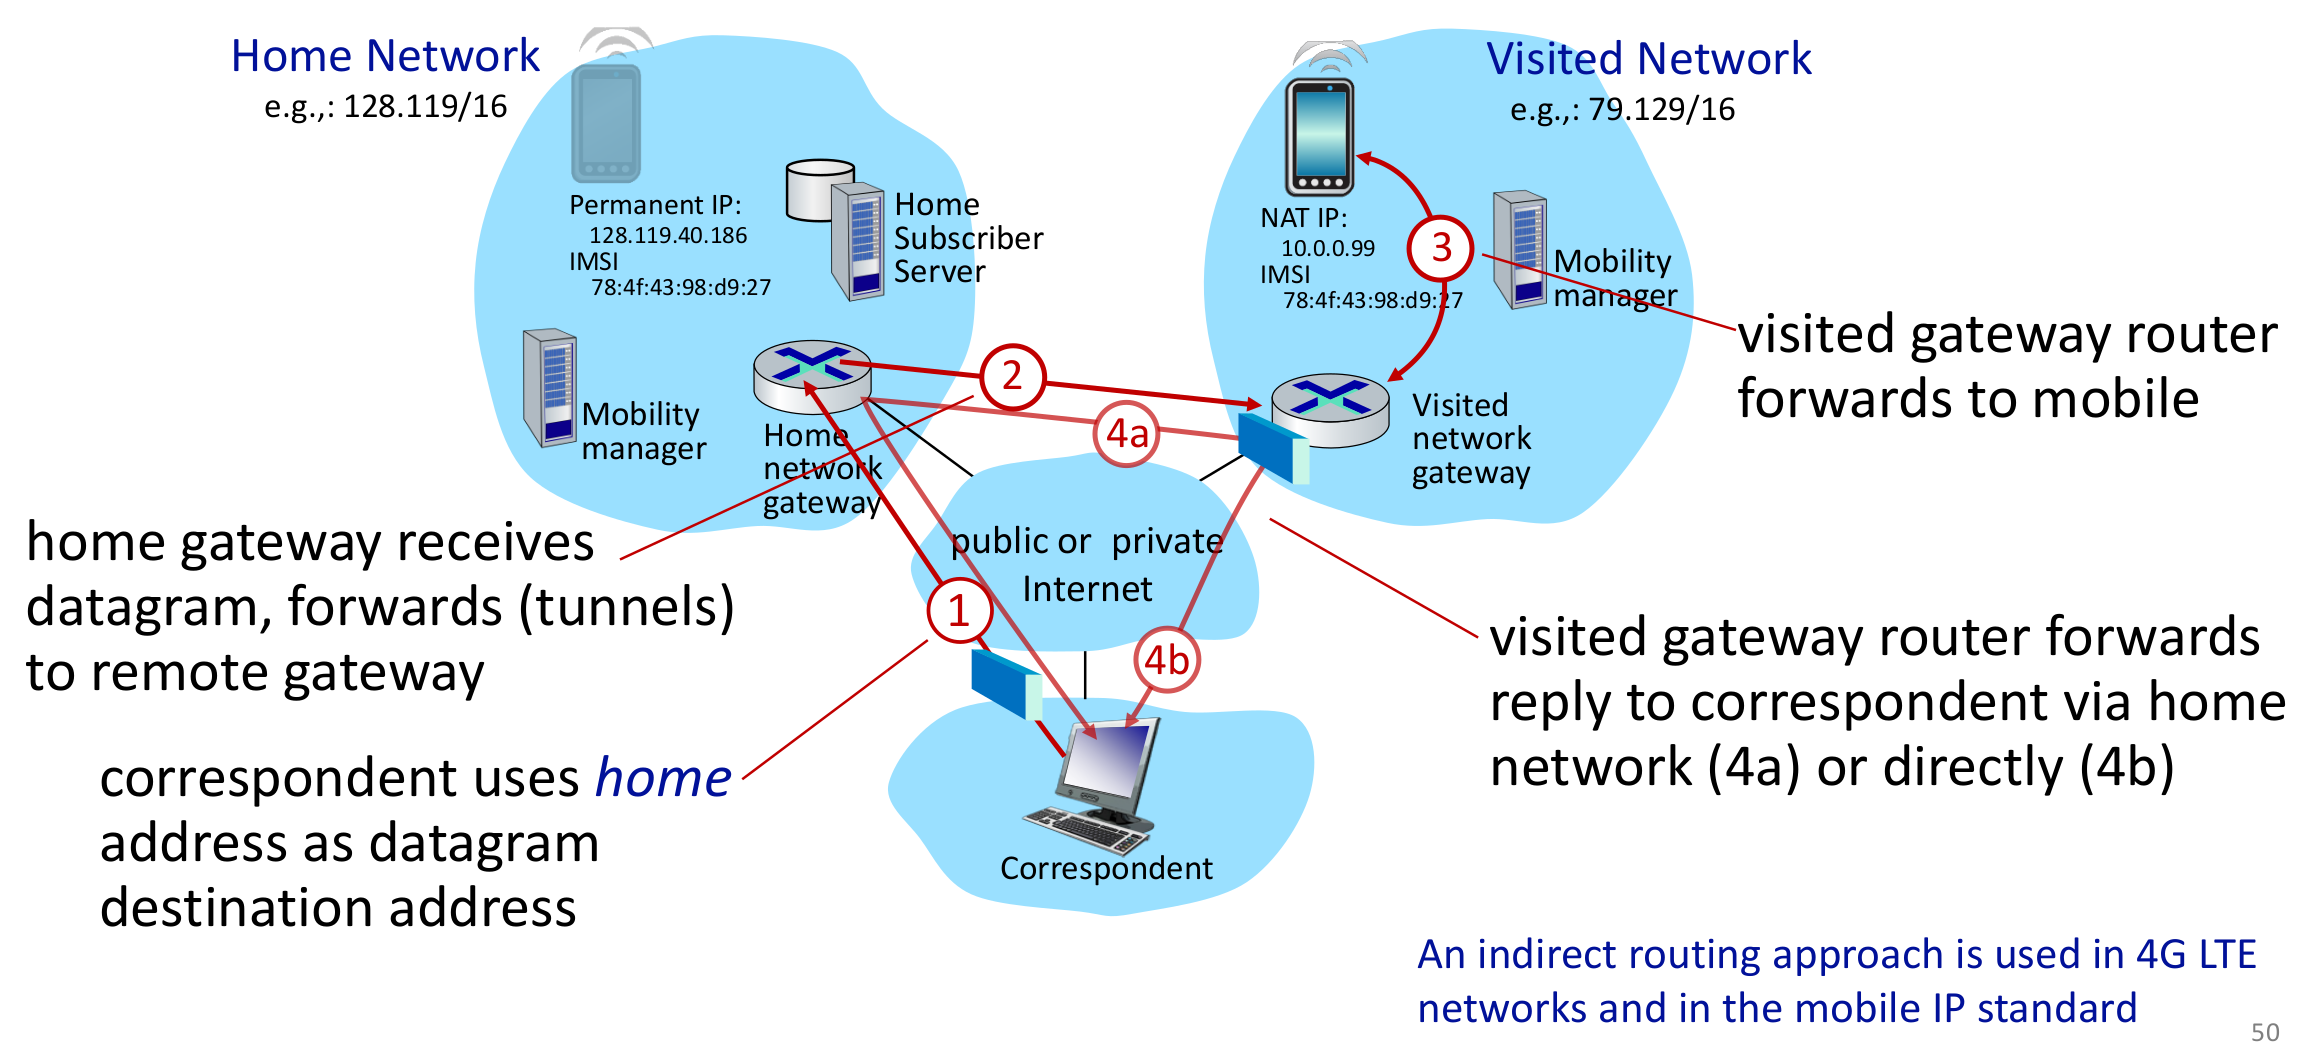
\includegraphics{images/mn_indirect.png}
   \caption{Indirect routing schema}
   \label{fig:mn_indirect}
\end{figure}

Once the mobile's location is known, the schema is fairly simple:
the sender sends the packet to the home network, which forwards it to the visited network, which in turn delivers it to the mobile device, lastly, the packet will be sent back to the sender, either directly or by using the same path.

To implement such solution, the requirements are:
\begin{itemize}
   \item Protocol to associate and disassociate a mobile to a visited network
   \item A protocol to Register the mobile's location in the HSS
   \item Tunnelling protocol to forward packets between the home and visited networks
   \begin{itemize}
      \item The home gateway performs encapsulation and forwarding of the correspondent’s original datagram
      \item On the receiving side, the gateway router performs decapsulation, NAT translation, and forwarding of the original datagram to the mobile device
   \end{itemize}
   
\end{itemize}

Indirect Routing is inefficient when mobile and sender are in the same network, but allows the mobility of the device to be \textbf{transparent} to the sender: ongoing connections (e.g. TCP) are not interrupted and can be maintained.

\subsection{Direct Routing}
\begin{figure}[htbp]
   \centering
   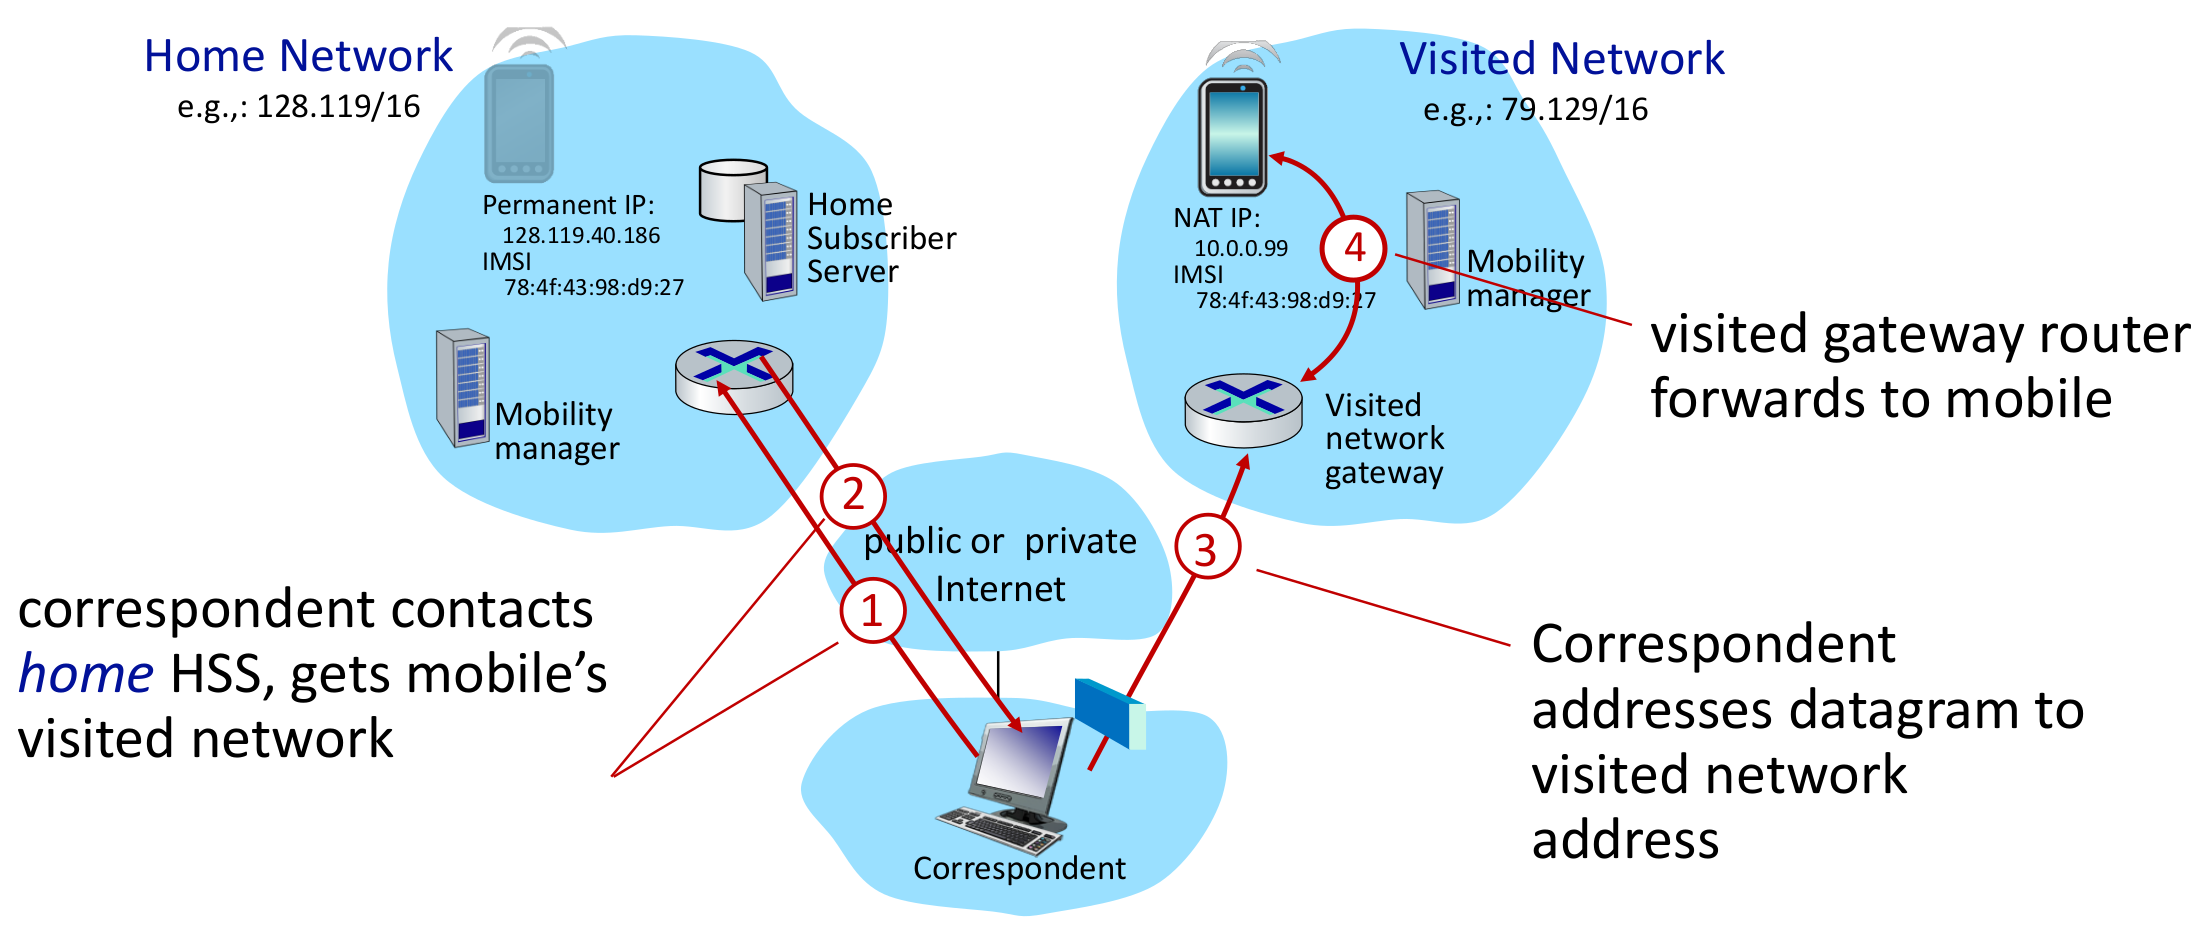
\includegraphics{images/mn_direct.png}
   \caption{Direct routing schema}
   \label{fig:mn_direct}
\end{figure}
As displayed in Fig. \ref{fig:mn_direct}, the main difference here is that the sender sends the packet directly to the mobile device, after receiving the foreign address from the home network.

This approach overcomes the inefficiency of the indirect routing, but it requires the sender to know the mobile's location, which may change multiple times, requiring the sender to ask the home network for the new location.

\subsection{Key-tasks in 4G Mobility}
\begin{figure}[htbp]
   \centering
   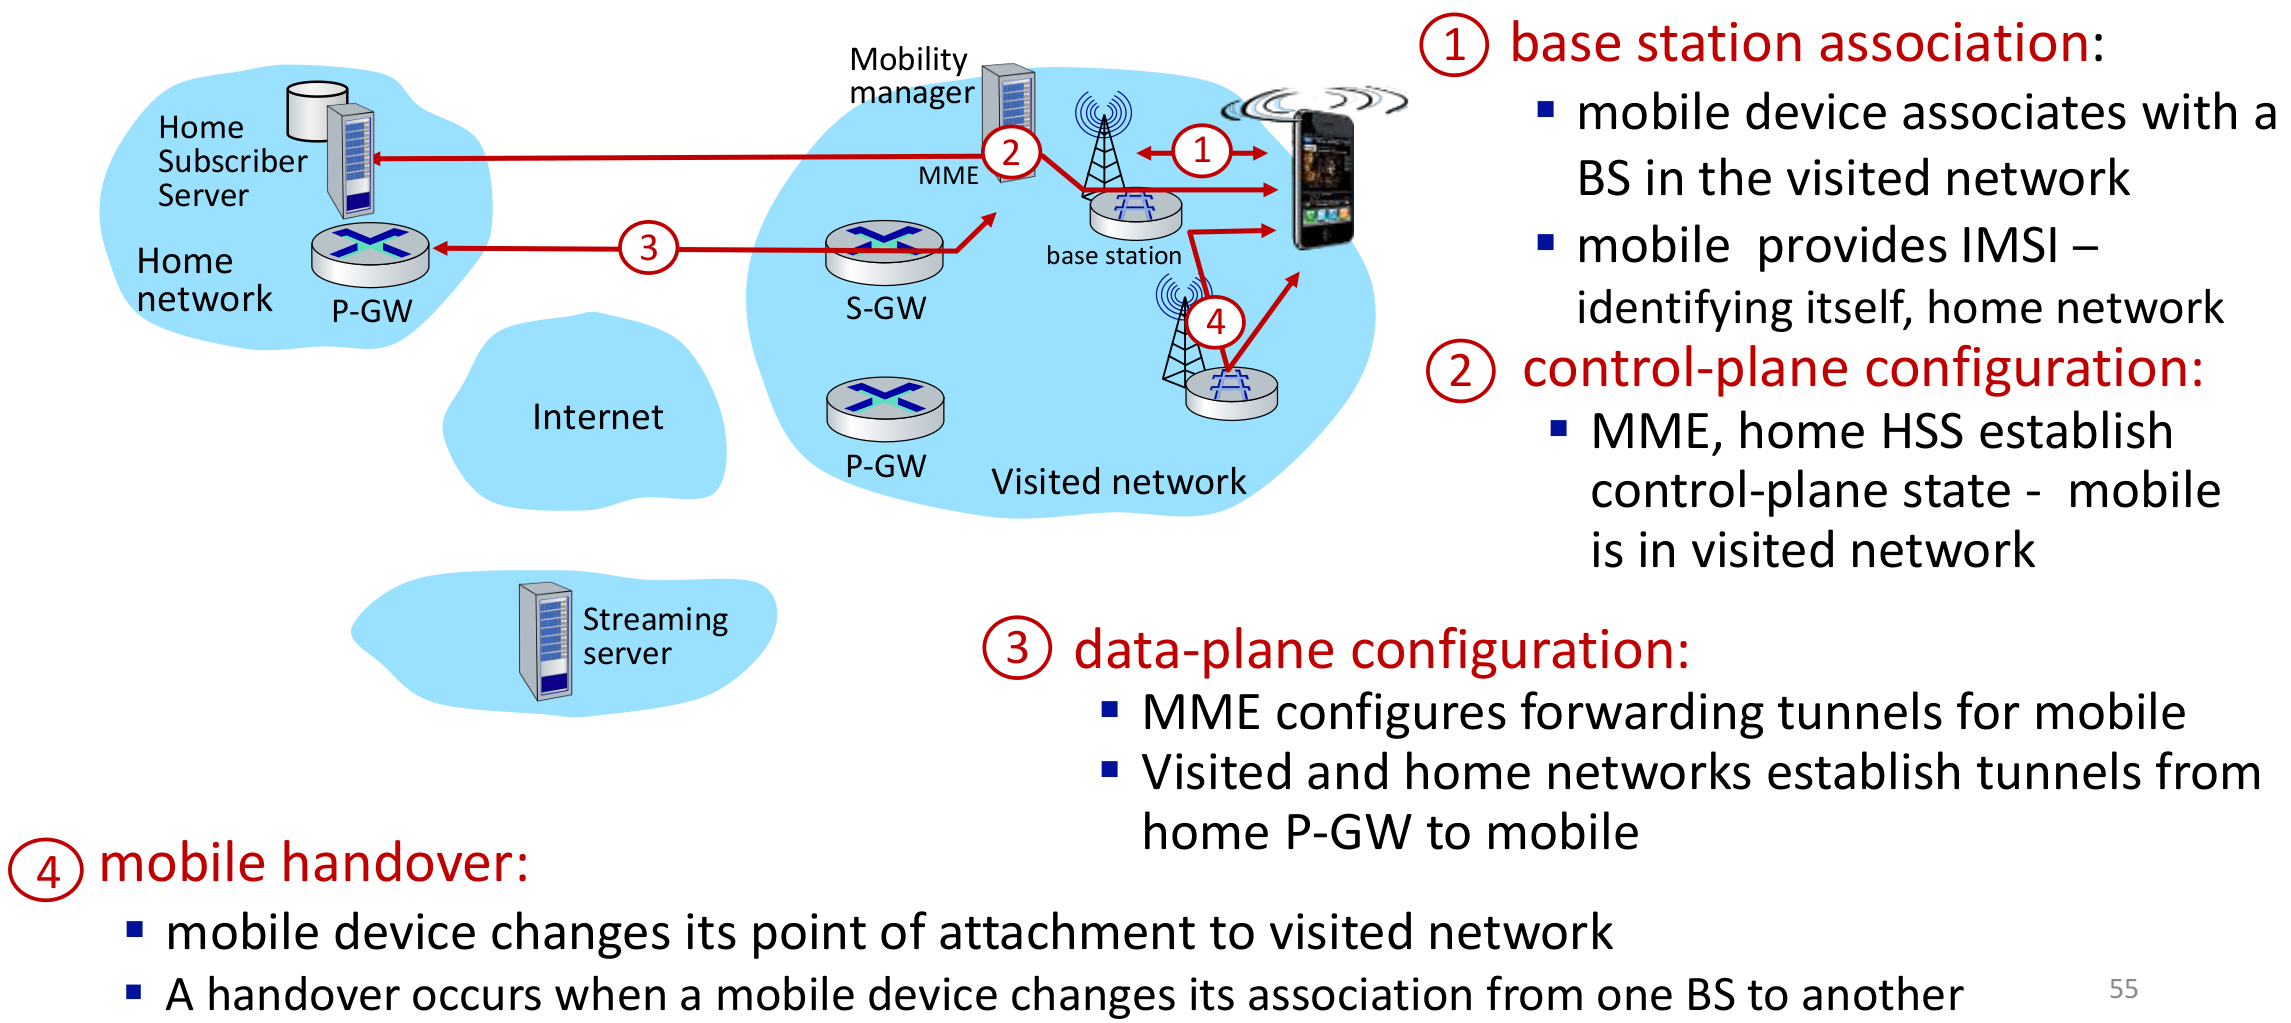
\includegraphics{images/4g_mobilitytasks.png}
   \caption{Mobility tasks}
   \label{fig:4g_mobilitytasks}
\end{figure}

\section{Handover in the same cellular network}
\begin{paracol}{2}
   \begin{figure}[htbp]
      \centering
      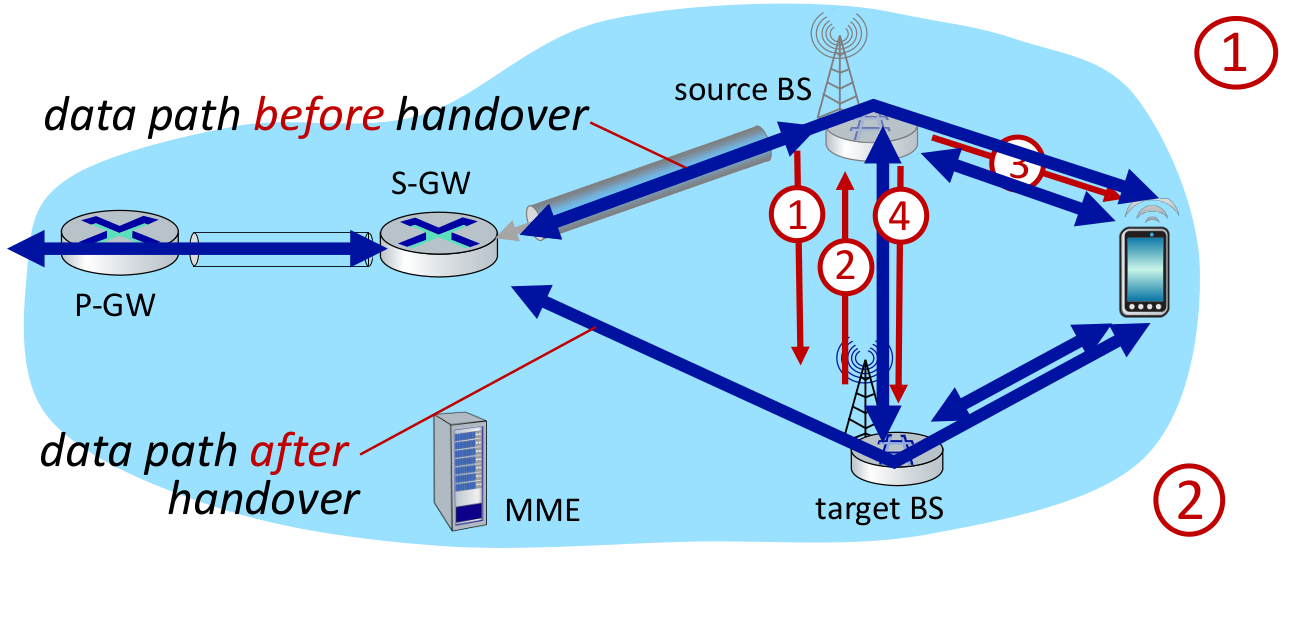
\includegraphics{images/4g_BSHO1.png}
      \caption{Handover pt. 1}
      \label{fig:4g_BSHO1}
   \end{figure}
   \switchcolumn
   \begin{enumerate}
      \item Current BS decides to perform handover and selects a \textit{target BS}, to whom sends a \texttt{handover request}.
      \begin{itemize}
         \item May happen due to a change in the signal strength, cell overloading or whatsoever
         \item Note that it's the BS that decides to perform the handover, not the mobile device
         \item \textit{On which criteria is the target BS selected?}
      \end{itemize}
      \item Target BS preallocates radio time slots and resources for the mobile device and sends a \texttt{handover ACK} to the current BS, appending info for the mobile device.
      \item Source BS notifies the device of the new BS using the information received from the target BS.\\
      From the mobile device's perspective, the handover is not transparent, but it gets completed with this third step.
      \item Source BS stops sending datagrams to mobile, and forwards incoming ones to the target BS.
   \end{enumerate}
\end{paracol}

\begin{paracol}{2}
   \begin{figure}[htbp]
      \centering
      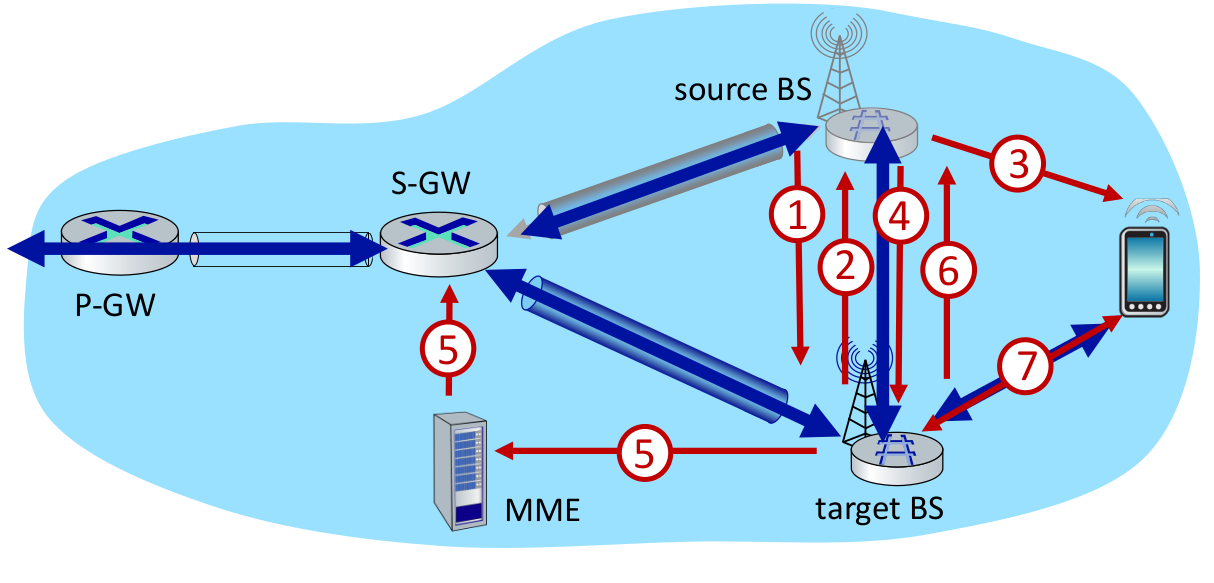
\includegraphics{images/4g_BSHO2.png}
      \caption{Handover pt. 2}
      \label{fig:4g_BSHO2}
   \end{figure}
   \switchcolumn
   \begin{enumerate}
      \setcounter{enumi}{4}
      \item Target BS informs the MME that it is the new serving BS for the mobile device, which in turn informs the SGW to update the path to the mobile device.
      \item Now target BS sends an \texttt{ACK} to the source BS, which can release resources and stop forwarding packets.
      \begin{itemize}
         \item \note{Shouldn't the target BS wait for an ACK by the MME?}
      \end{itemize}
      \item Datagrams now flow through the new channel from target BS to SGW.
   \end{enumerate}
\end{paracol}